% Created 2021-11-03 mié 11:39
% Intended LaTeX compiler: lualatex
\documentclass[table]{scrartcl}
\usepackage[left=1.5cm,right=1.5cm,bottom=2.5cm,letterpaper]{geometry}
\usepackage[spanish, es-nodecimaldot, es-tabla]{babel}
\usepackage[utf8]{inputenc}
\usepackage{blindtext}
\usepackage{multicol}
\usepackage{subfigure}
\usepackage[most]{tcolorbox}
\usepackage{etoolbox}
\usepackage{minted}
\usepackage{hyperref}
% \usepackage[table,xcdraw]{xcolor}
\usepackage{longtable}
\usepackage{multirow}
\usepackage[default]{comfortaa}
\usepackage[T1]{fontenc}

\usepackage{caption}
\usepackage{breqn}
\usemintedstyle{emacs}
\usepackage[ruled,vlined]{algorithm2e}
\newenvironment{code}{\captionsetup{type=listing}}{}
\definecolor{custom}{HTML}{F8F8F8}
\setminted{frame=lines,breaklines=true,bgcolor=custom,fontsize=\scriptsize,linenos}
\renewcommand\listoflistingscaption{Índice de \listingscaption\@s}
\renewcommand{\listingscaption}{Código}
\BeforeBeginEnvironment{listing}{\begin{code}}
  \AfterEndEnvironment{listing}{\end{code}}
\BeforeBeginEnvironment{minted}{\begin{code}}
  \AfterEndEnvironment{minted}{\end{code}}
\author{Monsalvo Bolaños Melissa Monserrat y Romero Andrade Cristian}
\date{\today}
\title{Practica 4}
\hypersetup{
  pdfauthor={Monsalvo Bolaños Melissa Monserrat y Romero Andrade Cristian},
  pdftitle={Practica 3},
  pdfkeywords={},
  pdfsubject={},
  pdfcreator={Emacs 27.2 (Org mode 9.6)},
  pdflang={English}}

\newcommand{\tituloTrabajo}{Practica No. 4\\Construcción de Máquinas de
  estados Usando Memorias Direccionamiento
  Entrada - Estado}
\newcommand{\fechaEntrega}{14 de octubre de 2021}

\usepackage{subfiles}
\usepackage[backend=biber,style=apa]{biblatex}
\addbibresource{../bib.bib}

\begin{document}
\begin{titlepage}
  \centering

    {\scshape{\Huge Facultad de Ingeniería\par{}}}\vspace{0.25cm}

    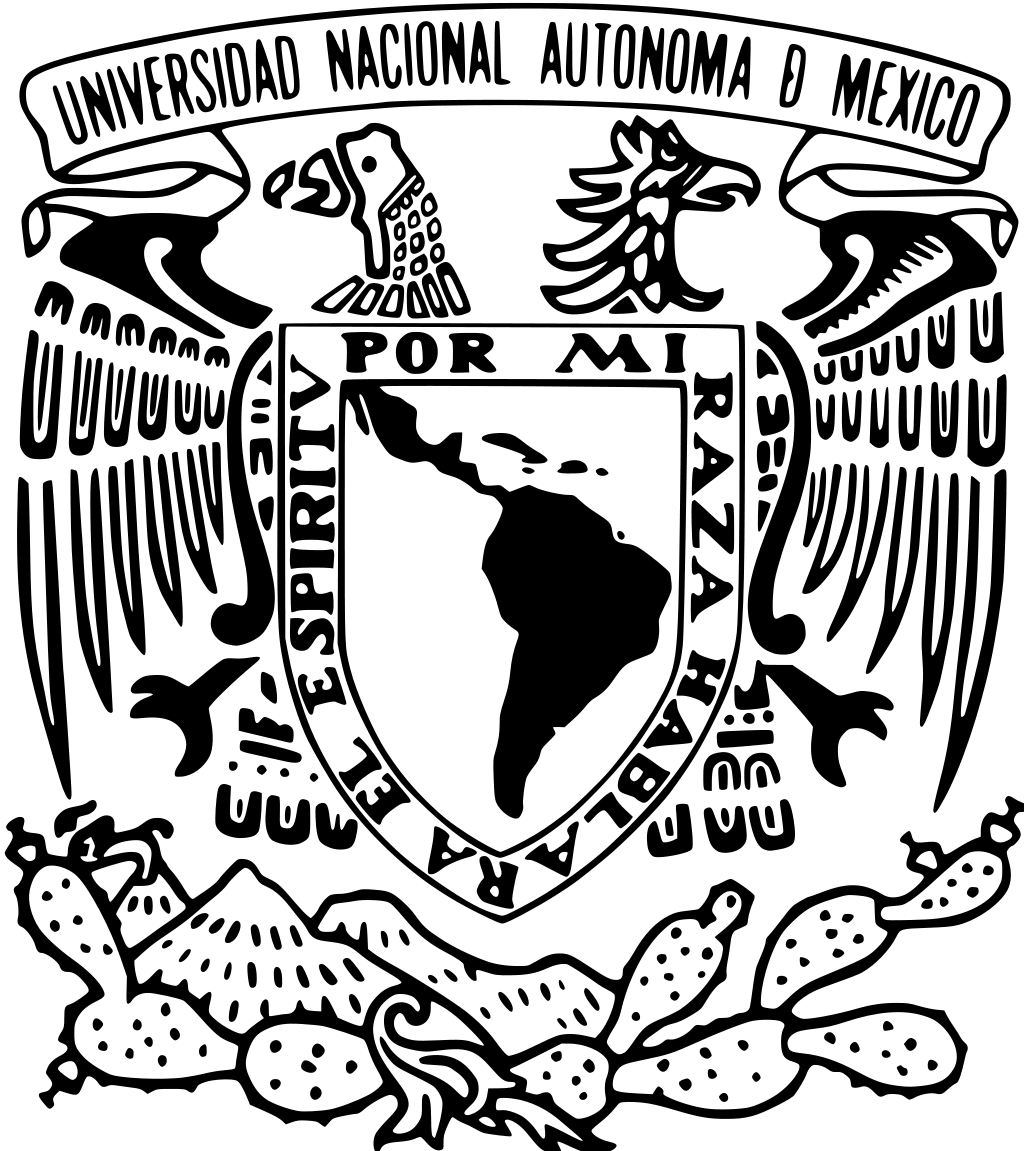
\includegraphics[width=0.25\textwidth]{../img_common/unam_logo}\vspace{0.5cm}

    {\scshape{\Large Lab. Organización y Arquitectura de Computadoras\par{}}}\vfill{}


    {\huge \textbf{\tituloTrabajo{}}}\vfill{}


    {\Large
      Alumnos
      \begin{itemize}

        \item Monsalvo Bolaños Melissa Monserrat

        \item Romero Andrade Cristian
      \end{itemize}
    }\vfill{}

      {\large Grupo: 01\par{}}\vfill{}

    {\large Profesor\\Ing.~Adrian Ulises Mercado Martinez}\vfill{}
    \vfil{}
    {\large Semestre\\\textbf{2022--1}}
    \vfill{}
    % {\large Fecha de Entrega\\\fechaEntrega}
    % \vfill{}
    
\includegraphics[width=0.1\textwidth]{../img_common/inge_logo}

\end{titlepage}

\maketitle{}
\tableofcontents{}
\section{Introducción}
\label{sec:org6bd500f}
El direccionamiento entrada-estado se restringe a cartas ASM con una sola
entrada por estado. Una nueva porción de la palabra de memoria contiene
una representación binaria de la entrada a probar en cada estado, esta parte
es llamada “PRUEBA”. Con esta representación binaria un selector de entrada
elige una de las variables de entrada. La parte de liga tiene dos estados
siguientes, encogiéndose uno por el selector de liga, en base a la entrada
seleccionada por la parte de prueba. Si el valor de la entrada seleccionada
por el selector de entradas es igual a cero, entonces el selector de liga elegirá
la liga falsa, en caso contrario se seleccionará la liga verdadera.
Este método tiene grandes ventajas como el ahorro de memoria, que
cuenta con pocos elementos de hardware y que representa un sistema muy
versátil.
\begin{figure}[htbp]
  \centering
  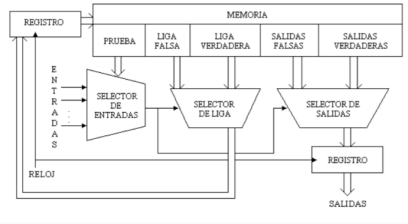
\includegraphics[width=0.6\textwidth]{./img/1.png}
  \caption{Direccionamiento Entrada-Estado}
\end{figure}
\newpage{}
\section{Objetivo}
\label{sec:org8bfa7f0}
Familiarizar al alumno en el conocimiento de construcción de máquinas de
estados usando direccionamiento de memorias con el método de
direccionamiento entrada--estado.

\section{Desarrollo}
\label{sec:orgac7043c}
Empezamos analizando siguiente figura, donde esta es una carta ASM
donde secuencialmente otorgamos los valores binarios de los estados y para
los estados de prueba
\begin{figure}[htbp]
  \centering
  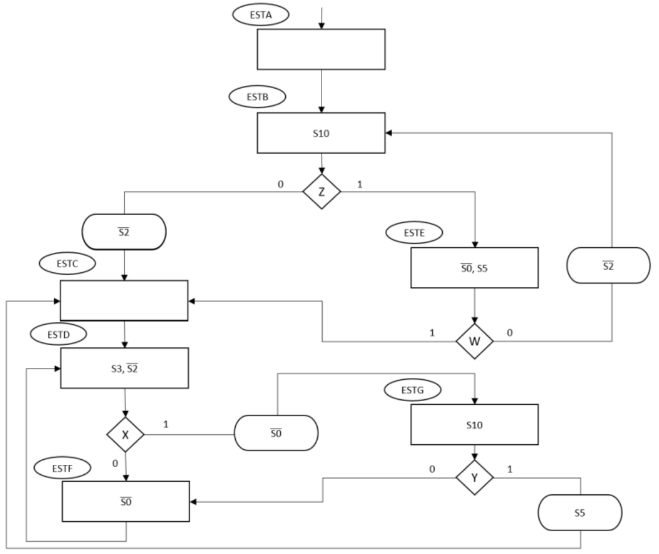
\includegraphics[width=0.4\textwidth]{./img/2.png}
  \caption{\label{fig:2}Carta ASM}
\end{figure}
\begin{center}
    \captionof{table}{Valores binarios a estados}\label{tab:1}
  \begin{tabular}{rl}
    \multicolumn{2}{c}{\cellcolor[HTML]{EA4335}{\color[HTML]{FFFFFF} \textbf{Entradas}}} \\
    ESTA & 000 \\
    ESTB & 001 \\
    ESTC & 010 \\
    ESTD & 011 \\
    ESTE & 100 \\
    ESTF & 101 \\
    ESTG & 110
\end{tabular}
\end{center}
\begin{center}
  \captionof{table}{Valores binarios de las entradas}\label{tab:2}
  \begin{tabular}{rl}
    \multicolumn{2}{c}{\cellcolor[HTML]{EA4335}{\color[HTML]{FFFFFF} \textbf{Prueba}}} \\
    x & 000 \\
    y & 001 \\
    z & 010 \\
    w & 011 \\
    aux & 100
  \end{tabular}
\end{center}
Una vez especificados nuestros estados y entradas, resolvemos la tabla de
verdad.
\begin{center}
  \captionof{table}{Tabla de verdad obtenida}\label{tab:3}
  \scriptsize
  \begin{longtable}{|ccc|ccccccccccccccccccc|}
\hline
\rowcolor[HTML]{CC4125}
\multicolumn{3}{|c|}{\cellcolor[HTML]{CC4125}{\color[HTML]{FFFFFF} \textbf{Dirección de memoria}}} & \multicolumn{19}{c|}{\cellcolor[HTML]{CC4125}Contenido de la memoria} \\ \hline
\rowcolor[HTML]{E06666}
\multicolumn{3}{|c|}{\cellcolor[HTML]{E06666}Estado Presente} & \multicolumn{3}{c|}{\cellcolor[HTML]{E06666}} & \multicolumn{3}{c|}{\cellcolor[HTML]{E06666}} & \multicolumn{3}{c|}{\cellcolor[HTML]{E06666}} & \multicolumn{5}{c|}{\cellcolor[HTML]{E06666}Salidas Falsas} & \multicolumn{5}{c|}{\cellcolor[HTML]{E06666}Salidas Verdaderas} \\ \cline{1-3} \cline{13-22}
\rowcolor[HTML]{F6B26B}
\multicolumn{1}{|c|}{\cellcolor[HTML]{F6B26B}Q2} & \multicolumn{1}{c|}{\cellcolor[HTML]{F6B26B}Q1} & Q0 & \multicolumn{3}{c|}{\multirow{-2}{*}{\cellcolor[HTML]{E06666}Prueba}} & \multicolumn{3}{c|}{\multirow{-2}{*}{\cellcolor[HTML]{E06666}Liga Falsa}} & \multicolumn{3}{c|}{\multirow{-2}{*}{\cellcolor[HTML]{E06666}Liga Verdadera}} & \multicolumn{1}{c|}{\cellcolor[HTML]{F6B26B}S5} & \multicolumn{1}{c|}{\cellcolor[HTML]{F6B26B}S3} & \multicolumn{1}{c|}{\cellcolor[HTML]{F6B26B}S2} & \multicolumn{1}{c|}{\cellcolor[HTML]{F6B26B}S1} & \multicolumn{1}{c|}{\cellcolor[HTML]{F6B26B}S0} & \multicolumn{1}{c|}{\cellcolor[HTML]{F6B26B}S5} & \multicolumn{1}{c|}{\cellcolor[HTML]{F6B26B}S3} & \multicolumn{1}{c|}{\cellcolor[HTML]{F6B26B}S2} & \multicolumn{1}{c|}{\cellcolor[HTML]{F6B26B}S1} & S0 \\ \hline
\rowcolor[HTML]{FFE599}
\multicolumn{1}{|c|}{\cellcolor[HTML]{FFE599}0} & \multicolumn{1}{c|}{\cellcolor[HTML]{FFE599}0} & 0 & \multicolumn{1}{c|}{\cellcolor[HTML]{FFE599}1} & \multicolumn{1}{c|}{\cellcolor[HTML]{FFE599}0} & \multicolumn{1}{c|}{\cellcolor[HTML]{FFE599}0} & \multicolumn{1}{c|}{\cellcolor[HTML]{FFE599}0} & \multicolumn{1}{c|}{\cellcolor[HTML]{FFE599}0} & \multicolumn{1}{c|}{\cellcolor[HTML]{FFE599}1} & \multicolumn{1}{c|}{\cellcolor[HTML]{FFE599}0} & \multicolumn{1}{c|}{\cellcolor[HTML]{FFE599}0} & \multicolumn{1}{c|}{\cellcolor[HTML]{FFE599}1} & \multicolumn{1}{c|}{\cellcolor[HTML]{FFE599}0} & \multicolumn{1}{c|}{\cellcolor[HTML]{FFE599}0} & \multicolumn{1}{c|}{\cellcolor[HTML]{FFE599}0} & \multicolumn{1}{c|}{\cellcolor[HTML]{FFE599}0} & \multicolumn{1}{c|}{\cellcolor[HTML]{FFE599}0} & \multicolumn{1}{c|}{\cellcolor[HTML]{FFE599}0} & \multicolumn{1}{c|}{\cellcolor[HTML]{FFE599}0} & \multicolumn{1}{c|}{\cellcolor[HTML]{FFE599}0} & \multicolumn{1}{c|}{\cellcolor[HTML]{FFE599}0} & 0 \\ \hline
\rowcolor[HTML]{B6D7A8}
\multicolumn{1}{|c|}{\cellcolor[HTML]{B6D7A8}0} & \multicolumn{1}{c|}{\cellcolor[HTML]{B6D7A8}0} & 1 & \multicolumn{1}{c|}{\cellcolor[HTML]{B6D7A8}0} & \multicolumn{1}{c|}{\cellcolor[HTML]{B6D7A8}1} & \multicolumn{1}{c|}{\cellcolor[HTML]{B6D7A8}0} & \multicolumn{1}{c|}{\cellcolor[HTML]{B6D7A8}0} & \multicolumn{1}{c|}{\cellcolor[HTML]{B6D7A8}1} & \multicolumn{1}{c|}{\cellcolor[HTML]{B6D7A8}0} & \multicolumn{1}{c|}{\cellcolor[HTML]{B6D7A8}1} & \multicolumn{1}{c|}{\cellcolor[HTML]{B6D7A8}0} & \multicolumn{1}{c|}{\cellcolor[HTML]{B6D7A8}0} & \multicolumn{1}{c|}{\cellcolor[HTML]{B6D7A8}0} & \multicolumn{1}{c|}{\cellcolor[HTML]{B6D7A8}0} & \multicolumn{1}{c|}{\cellcolor[HTML]{B6D7A8}0} & \multicolumn{1}{c|}{\cellcolor[HTML]{B6D7A8}1} & \multicolumn{1}{c|}{\cellcolor[HTML]{B6D7A8}0} & \multicolumn{1}{c|}{\cellcolor[HTML]{B6D7A8}0} & \multicolumn{1}{c|}{\cellcolor[HTML]{B6D7A8}0} & \multicolumn{1}{c|}{\cellcolor[HTML]{B6D7A8}0} & \multicolumn{1}{c|}{\cellcolor[HTML]{B6D7A8}1} & 0 \\ \hline
\rowcolor[HTML]{A2C4C9}
\multicolumn{1}{|c|}{\cellcolor[HTML]{A2C4C9}0} & \multicolumn{1}{c|}{\cellcolor[HTML]{A2C4C9}1} & 0 & \multicolumn{1}{c|}{\cellcolor[HTML]{A2C4C9}1} & \multicolumn{1}{c|}{\cellcolor[HTML]{A2C4C9}0} & \multicolumn{1}{c|}{\cellcolor[HTML]{A2C4C9}0} & \multicolumn{1}{c|}{\cellcolor[HTML]{A2C4C9}0} & \multicolumn{1}{c|}{\cellcolor[HTML]{A2C4C9}1} & \multicolumn{1}{c|}{\cellcolor[HTML]{A2C4C9}1} & \multicolumn{1}{c|}{\cellcolor[HTML]{A2C4C9}0} & \multicolumn{1}{c|}{\cellcolor[HTML]{A2C4C9}1} & \multicolumn{1}{c|}{\cellcolor[HTML]{A2C4C9}1} & \multicolumn{1}{c|}{\cellcolor[HTML]{A2C4C9}0} & \multicolumn{1}{c|}{\cellcolor[HTML]{A2C4C9}0} & \multicolumn{1}{c|}{\cellcolor[HTML]{A2C4C9}0} & \multicolumn{1}{c|}{\cellcolor[HTML]{A2C4C9}0} & \multicolumn{1}{c|}{\cellcolor[HTML]{A2C4C9}0} & \multicolumn{1}{c|}{\cellcolor[HTML]{A2C4C9}0} & \multicolumn{1}{c|}{\cellcolor[HTML]{A2C4C9}0} & \multicolumn{1}{c|}{\cellcolor[HTML]{A2C4C9}0} & \multicolumn{1}{c|}{\cellcolor[HTML]{A2C4C9}0} & 0 \\ \hline
\rowcolor[HTML]{A4C2F4}
\multicolumn{1}{|c|}{\cellcolor[HTML]{A4C2F4}0} & \multicolumn{1}{c|}{\cellcolor[HTML]{A4C2F4}1} & 1 & \multicolumn{1}{c|}{\cellcolor[HTML]{A4C2F4}0} & \multicolumn{1}{c|}{\cellcolor[HTML]{A4C2F4}0} & \multicolumn{1}{c|}{\cellcolor[HTML]{A4C2F4}0} & \multicolumn{1}{c|}{\cellcolor[HTML]{A4C2F4}1} & \multicolumn{1}{c|}{\cellcolor[HTML]{A4C2F4}0} & \multicolumn{1}{c|}{\cellcolor[HTML]{A4C2F4}1} & \multicolumn{1}{c|}{\cellcolor[HTML]{A4C2F4}1} & \multicolumn{1}{c|}{\cellcolor[HTML]{A4C2F4}1} & \multicolumn{1}{c|}{\cellcolor[HTML]{A4C2F4}0} & \multicolumn{1}{c|}{\cellcolor[HTML]{A4C2F4}0} & \multicolumn{1}{c|}{\cellcolor[HTML]{A4C2F4}1} & \multicolumn{1}{c|}{\cellcolor[HTML]{A4C2F4}0} & \multicolumn{1}{c|}{\cellcolor[HTML]{A4C2F4}0} & \multicolumn{1}{c|}{\cellcolor[HTML]{A4C2F4}0} & \multicolumn{1}{c|}{\cellcolor[HTML]{A4C2F4}0} & \multicolumn{1}{c|}{\cellcolor[HTML]{A4C2F4}1} & \multicolumn{1}{c|}{\cellcolor[HTML]{A4C2F4}0} & \multicolumn{1}{c|}{\cellcolor[HTML]{A4C2F4}0} & 0 \\ \hline
\rowcolor[HTML]{9FC5E8}
\multicolumn{1}{|c|}{\cellcolor[HTML]{9FC5E8}1} & \multicolumn{1}{c|}{\cellcolor[HTML]{9FC5E8}0} & 0 & \multicolumn{1}{c|}{\cellcolor[HTML]{9FC5E8}0} & \multicolumn{1}{c|}{\cellcolor[HTML]{9FC5E8}1} & \multicolumn{1}{c|}{\cellcolor[HTML]{9FC5E8}1} & \multicolumn{1}{c|}{\cellcolor[HTML]{9FC5E8}0} & \multicolumn{1}{c|}{\cellcolor[HTML]{9FC5E8}0} & \multicolumn{1}{c|}{\cellcolor[HTML]{9FC5E8}1} & \multicolumn{1}{c|}{\cellcolor[HTML]{9FC5E8}0} & \multicolumn{1}{c|}{\cellcolor[HTML]{9FC5E8}1} & \multicolumn{1}{c|}{\cellcolor[HTML]{9FC5E8}0} & \multicolumn{1}{c|}{\cellcolor[HTML]{9FC5E8}1} & \multicolumn{1}{c|}{\cellcolor[HTML]{9FC5E8}0} & \multicolumn{1}{c|}{\cellcolor[HTML]{9FC5E8}0} & \multicolumn{1}{c|}{\cellcolor[HTML]{9FC5E8}0} & \multicolumn{1}{c|}{\cellcolor[HTML]{9FC5E8}0} & \multicolumn{1}{c|}{\cellcolor[HTML]{9FC5E8}1} & \multicolumn{1}{c|}{\cellcolor[HTML]{9FC5E8}0} & \multicolumn{1}{c|}{\cellcolor[HTML]{9FC5E8}0} & \multicolumn{1}{c|}{\cellcolor[HTML]{9FC5E8}0} & 0 \\ \hline
\rowcolor[HTML]{B4A7D6}
\multicolumn{1}{|c|}{\cellcolor[HTML]{B4A7D6}1} & \multicolumn{1}{c|}{\cellcolor[HTML]{B4A7D6}0} & 1 & \multicolumn{1}{c|}{\cellcolor[HTML]{B4A7D6}1} & \multicolumn{1}{c|}{\cellcolor[HTML]{B4A7D6}0} & \multicolumn{1}{c|}{\cellcolor[HTML]{B4A7D6}0} & \multicolumn{1}{c|}{\cellcolor[HTML]{B4A7D6}0} & \multicolumn{1}{c|}{\cellcolor[HTML]{B4A7D6}1} & \multicolumn{1}{c|}{\cellcolor[HTML]{B4A7D6}1} & \multicolumn{1}{c|}{\cellcolor[HTML]{B4A7D6}0} & \multicolumn{1}{c|}{\cellcolor[HTML]{B4A7D6}1} & \multicolumn{1}{c|}{\cellcolor[HTML]{B4A7D6}1} & \multicolumn{1}{c|}{\cellcolor[HTML]{B4A7D6}0} & \multicolumn{1}{c|}{\cellcolor[HTML]{B4A7D6}0} & \multicolumn{1}{c|}{\cellcolor[HTML]{B4A7D6}0} & \multicolumn{1}{c|}{\cellcolor[HTML]{B4A7D6}0} & \multicolumn{1}{c|}{\cellcolor[HTML]{B4A7D6}0} & \multicolumn{1}{c|}{\cellcolor[HTML]{B4A7D6}0} & \multicolumn{1}{c|}{\cellcolor[HTML]{B4A7D6}0} & \multicolumn{1}{c|}{\cellcolor[HTML]{B4A7D6}0} & \multicolumn{1}{c|}{\cellcolor[HTML]{B4A7D6}0} & 0 \\ \hline
\rowcolor[HTML]{D5A6BD}
\multicolumn{1}{|c|}{\cellcolor[HTML]{D5A6BD}1} & \multicolumn{1}{c|}{\cellcolor[HTML]{D5A6BD}1} & 0 & \multicolumn{1}{c|}{\cellcolor[HTML]{D5A6BD}0} & \multicolumn{1}{c|}{\cellcolor[HTML]{D5A6BD}0} & \multicolumn{1}{c|}{\cellcolor[HTML]{D5A6BD}1} & \multicolumn{1}{c|}{\cellcolor[HTML]{D5A6BD}1} & \multicolumn{1}{c|}{\cellcolor[HTML]{D5A6BD}0} & \multicolumn{1}{c|}{\cellcolor[HTML]{D5A6BD}1} & \multicolumn{1}{c|}{\cellcolor[HTML]{D5A6BD}0} & \multicolumn{1}{c|}{\cellcolor[HTML]{D5A6BD}1} & \multicolumn{1}{c|}{\cellcolor[HTML]{D5A6BD}0} & \multicolumn{1}{c|}{\cellcolor[HTML]{D5A6BD}0} & \multicolumn{1}{c|}{\cellcolor[HTML]{D5A6BD}0} & \multicolumn{1}{c|}{\cellcolor[HTML]{D5A6BD}0} & \multicolumn{1}{c|}{\cellcolor[HTML]{D5A6BD}1} & \multicolumn{1}{c|}{\cellcolor[HTML]{D5A6BD}0} & \multicolumn{1}{c|}{\cellcolor[HTML]{D5A6BD}1} & \multicolumn{1}{c|}{\cellcolor[HTML]{D5A6BD}0} & \multicolumn{1}{c|}{\cellcolor[HTML]{D5A6BD}0} & \multicolumn{1}{c|}{\cellcolor[HTML]{D5A6BD}1} & 0 \\ \hline
\end{longtable}

\end{center}
Con los valores obtenidos, implementamos la memoria en Quartus con la
programación VHDL obteniendo el siguiente código:
\begin{code}
  \inputminted{vhdl}{./rom.vhd}
  \caption{\texttt{rom.vhd}}
\end{code}
A continuación escribimos el bloque que realiza el direccionamiento
entrada-estado.
\begin{code}
  \inputminted{vhdl}{./registro_entrada.vhd}
  \caption{\texttt{registro_entrada.vhd}}
\end{code}
\begin{code}
  \inputminted{vhdl}{./registro_salida.vhd}
  \caption{\texttt{registro_salida.vhd}}
\end{code}
Ahora escribimos el separador de datos almacenados en memoria para así
asignar el estado siguiente, valor de prueba, ligas falsas y las ligas
verdaderas, donde estas dos últimas son la salida del bloque.
\begin{code}
  \inputminted{vhdl}{./separador.vhd}
  \caption{\texttt{separador.vhd}}
\end{code}
Para realizar la elección correcta de las salidas, teniendo en cuenta el valor
de las entradas, se generó el selector de entrada para poder enviar un valor
binario correspondiente a cada entrada; El selector de la liga también se
generó para poder elegir entre una liga falsa o una liga real, y, por lo tanto, un
selector de inicio para obtener un rendimiento adecuado de acuerdo con la
liga que ha ocurrido
\begin{code}
  \inputminted{vhdl}{./selector_entrada.vhd}
  \caption{\texttt{selector_entrada.vhd}}
\end{code}
\begin{code}
  \inputminted{vhdl}{./selector_liga.vhd}
  \caption{\texttt{selector_liga.vhd}}
\end{code}
\begin{code}
  \inputminted{vhdl}{./selector_salida.vhd}
  \caption{\texttt{selector_salida.vhd}}
\end{code}
\newpage{}
\subsection{Diagrama}\label{sec:diagrama}
\begin{figure}[htbp]
  \centering
  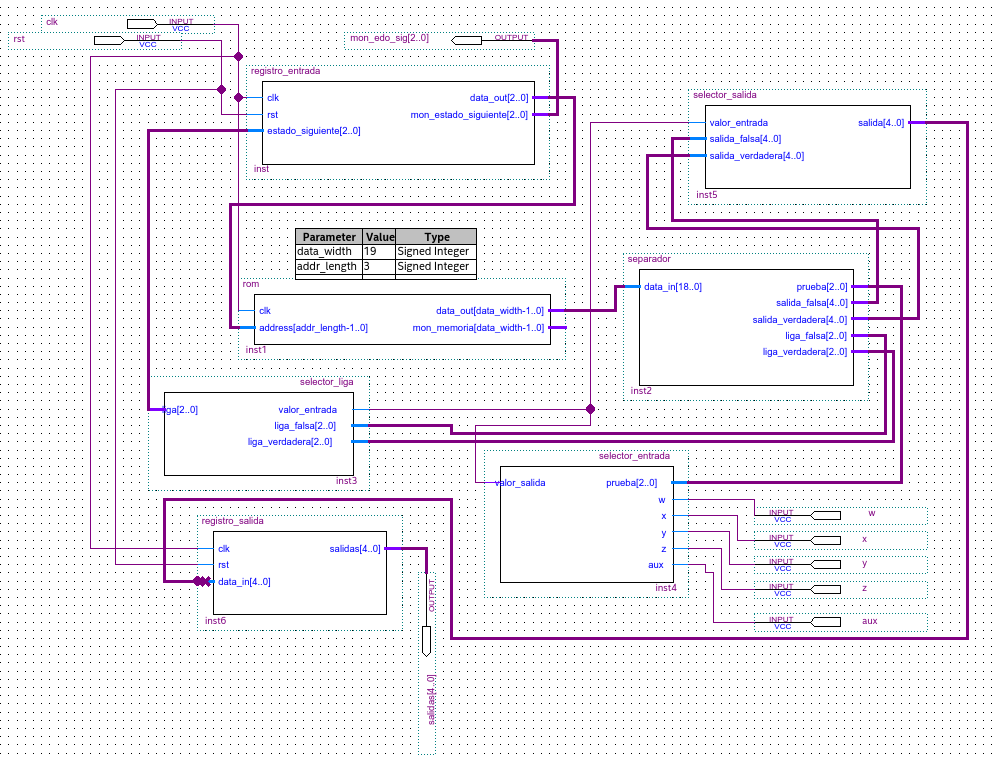
\includegraphics[width=\textwidth]{./img/dia.png}
  \caption{Diagrama de Bloques}
\end{figure}

\subsection{Simulación}\label{sec:simulacion}
Una vez obtenido el diagrama esquemático proseguimos con la simulación.
Para el siguiente ejemplo se considera que todas las entradas están en 0
menos W.

Sigamos la trayectoria en la carta ASM. Empezamos en el estado A y
pasamos al B, en este primer caso, la salida corresponde a 00000.
Posteriormente en el estado B se evalúa Z y pasa al estado C, este paso tiene
como salida en alto a s1.

El siguiente paso es del estado C al D con salida $00000$. Posteriormente, en
el estado D se evalúa X, como está en 0 pasa al estado F y solo se activa s3.

Por último, del estado F regresa al estado D con ninguna salida en alto y como
X no cambia su valor, se queda en un ciclo.
\begin{figure}[htbp]
  \centering
  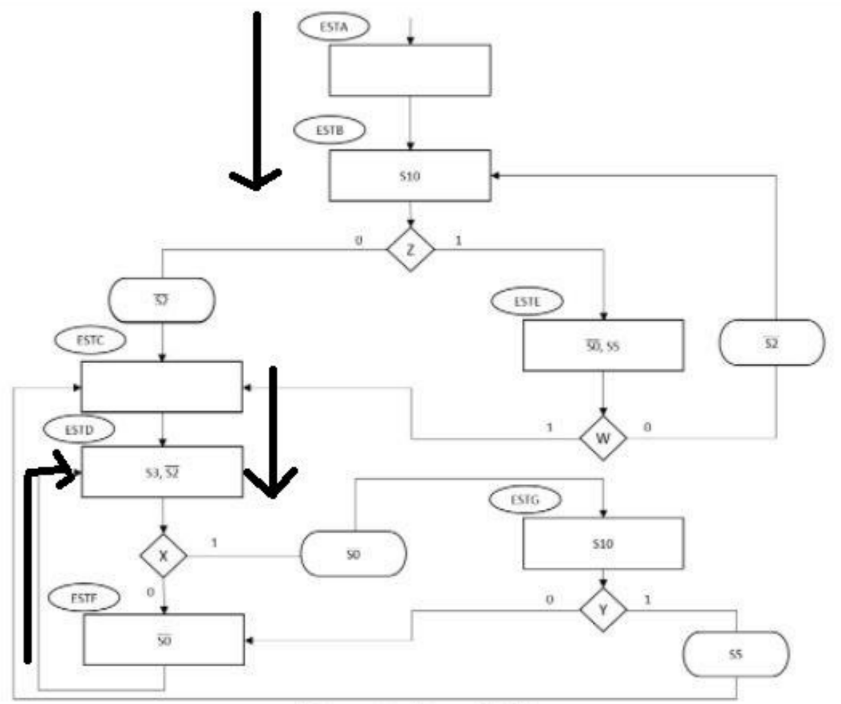
\includegraphics[width=0.6\textwidth]{./img/ruta.png}
  \caption{Ruta Carta ASM}
\end{figure}
\begin{figure}[htbp]
  \centering
  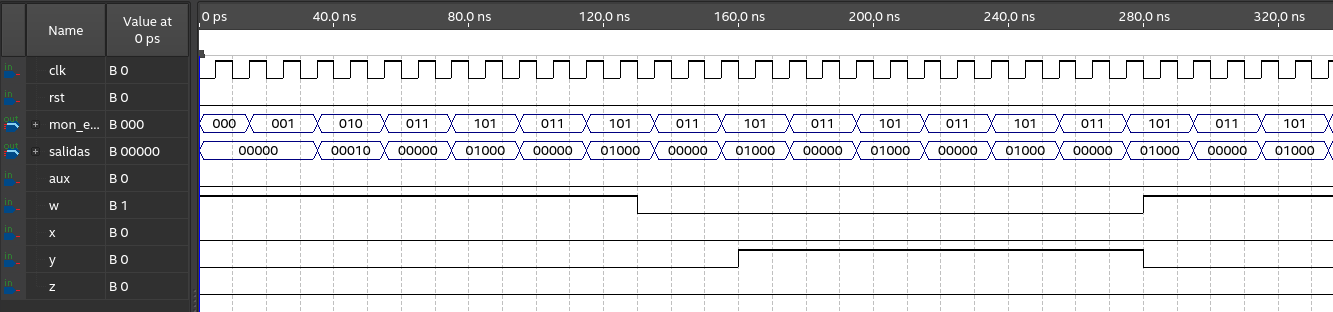
\includegraphics[width=\textwidth]{./img/sim.png}
  \caption{Simulación}
\end{figure}

\section{Conclusiones}
\label{sec:orgdab2190}

\subsection*{Monsalvo Bolaños Melissa Monserrat}\label{sec:mons-bolan-melissa}

Con el desarrollo de esta práctica pudimos implementar la aplicación de una
carta ASM por el método de direccionamiento de entrada estado. Pudimos
observar que, a diferencia del método de direccionamiento por trayectoria,
este método requiere de más elementos. Y pudimos percatarnos de que a
diferencia del método anterior aquí no podemos evaluar múltiples entradas,
sin embargo observamos las bondades que nos ofrece, como la significativa
reducción en la memoria.

\subsection*{Romero Andrade Cristian}
\label{sec:romero-andr-crist}

La implementación de la carta ASM usando direccionamiento estrada-estado
fue sencilla puesto que el uso de memorias “traduce” la tabla de verdad que se
obtuvo al resolver la carta. Consecuentemente se logró desarrollar los bloques
en código vhdl para lograr que concuerde la simulación con la carta y asu vez
la tabla de verdad

\subsection*{Conclusiones en equipo}\label{sec:concl-en-equipo}

En la presente se logró implementar en VHDL la carta ASM usando
direccionamiento entrada-estado, en mayor parte se utilizó el mismo diseño
de la práctica anterior con unos cambios como por ejemplo la selección de
liga y el de salidas para poder implementar dicho direccionamiento.

\nocite{*}
\addcontentsline{toc}{section}{Referencias}
\printbibliography{}
\newpage{}

\listoftables{}
\listoffigures{}
\listoflistings{}
\end{document}
